\documentclass[12pt]{article}
\usepackage[utf8]{inputenc}
\usepackage{booktabs}
\usepackage{geometry}
\usepackage{graphicx}
\geometry{a4paper, margin=1in}
\title{Results of the Fisher Combined Test}
\author{Sara Fraija}
\date{\today}
\begin{document}
\maketitle
\section{Resultados}

\begin{table}[h!]
\centering
\resizebox{\textwidth}{!}{%
\begin{tabular}{l c c c c c c}
\toprule
\textbf{GRB} & \textbf{Transit} & \textbf{Significance} & \textbf{Significance Corregida} & \textbf{p-value} & \textbf{Corrected p-value} & \textbf{PDF} \\ \midrule
GRB170708046 & 1__plus_20 & 0.82 & 0.07 & 7.939e-01 & 4.733e-01 & 7.150e-01 \\
GRB170816599 & 1__plus_20 & 1.72 & 1.20 & 9.573e-01 & 1.142e-01 & 9.091e-01 \\
GRB170222209 & 1__plus_20 & 0.00 & -2.45 & 5.000e-01 & 9.928e-01 & 6.011e-01 \\
GRB170403583 & 1__plus_20 & 0.47 & -1.16 & 6.808e-01 & 8.767e-01 & 6.428e-01 \\
GRB170826369 & 1__plus_20 & 2.18 & 1.21 & 9.854e-01 & 1.131e-01 & 9.629e-01 \\
GRB190515190 & 1__plus_20 & 0.00 & -2.92 & 5.000e-01 & 9.982e-01 & 6.011e-01 \\
GRB150101270 & 1__plus_20 & 1.75 & 1.75 & 9.599e-01 & 4.006e-02 & 9.137e-01 \\
GRB150101641 & 1__plus_20 & 1.09 & 1.09 & 8.621e-01 & 1.379e-01 & 7.797e-01 \\
GRB150110923 & 1__plus_20 & 1.50 & 1.50 & 9.332e-01 & 6.681e-02 & 8.705e-01 \\
GRB150120123 & 1__plus_20 & 0.26 & 0.26 & 6.026e-01 & 3.974e-01 & 6.143e-01 \\
GRB150922234 & 1__plus_20 & 0.00 & -0.00 & 5.000e-01 & 5.000e-01 & 6.011e-01 \\
GRB151228129 & 1__plus_20 & 0.79 & 0.79 & 7.852e-01 & 2.148e-01 & 7.080e-01 \\
GRB151229285 & 1__plus_20 & 0.07 & 0.07 & 5.279e-01 & 4.721e-01 & 6.020e-01 \\
GRB160612842 & 1__plus_20 & 0.00 & -0.00 & 5.000e-01 & 5.000e-01 & 6.011e-01 \\
GRB160624477 & 1__plus_20 & 1.64 & 1.64 & 9.495e-01 & 5.050e-02 & 8.960e-01 \\
GRB160726065 & 1__plus_20 & 1.59 & 1.59 & 9.441e-01 & 5.592e-02 & 8.873e-01 \\
GRB170318644 & 1__plus_20 & 0.64 & 0.64 & 7.389e-01 & 2.611e-01 & 6.749e-01 \\
GRB170325331 & 1__plus_20 & 1.42 & 1.42 & 9.222e-01 & 7.780e-02 & 8.544e-01 \\
GRB170803729 & 1__plus_20 & 0.00 & -0.00 & 5.000e-01 & 5.000e-01 & 6.011e-01 \\
GRB170817529 & 1__plus_20 & 1.31 & 1.31 & 9.049e-01 & 9.510e-02 & 8.309e-01 \\
GRB180204109 & 1__plus_20 & 2.40 & 2.40 & 9.918e-01 & 8.198e-03 & 9.776e-01 \\
GRB180418281 & 1__plus_20 & 0.41 & 0.41 & 6.591e-01 & 3.409e-01 & 6.332e-01 \\
GRB180715755 & 1__plus_20 & 0.58 & 0.58 & 7.190e-01 & 2.810e-01 & 6.628e-01 \\
GRB180718082 & 1__plus_20 & 1.70 & 1.70 & 9.554e-01 & 4.457e-02 & 9.060e-01 \\
GRB180805543 & 1__plus_20 & 2.65 & 2.65 & 9.960e-01 & 4.025e-03 & 9.881e-01 \\
GRB181125371 & 1__plus_20 & 1.33 & 1.33 & 9.082e-01 & 9.176e-02 & 8.353e-01 \\
GRB190427190 & 1__plus_20 & 2.44 & 2.44 & 9.927e-01 & 7.344e-03 & 9.797e-01 \\
GRB201008443 & 1__plus_20 & 1.90 & 1.90 & 9.713e-01 & 2.872e-02 & 9.344e-01 \\
GRB201214672 & 1__plus_20 & 0.57 & 0.57 & 7.157e-01 & 2.843e-01 & 6.609e-01 \\
GRB210323918 & 1__plus_20 & 1.39 & 1.39 & 9.177e-01 & 8.226e-02 & 8.482e-01 \\
GRB211024065 & 1__plus_20 & 0.48 & 0.48 & 6.844e-01 & 3.156e-01 & 6.445e-01 \\
GRB220412713 & 1__plus_20 & 1.53 & 1.53 & 9.370e-01 & 6.301e-02 & 8.762e-01 \\
GRB220418720 & 1__plus_20 & 2.13 & 2.13 & 9.834e-01 & 1.659e-02 & 9.587e-01 \\
GRB220511571 & 1__plus_20 & 1.05 & 1.05 & 8.531e-01 & 1.469e-01 & 7.701e-01 \\
GRB220617772 & 1__plus_20 & 2.46 & 2.46 & 9.931e-01 & 6.947e-03 & 9.806e-01 \\
GRB221120895 & 1__plus_20 & 0.00 & -0.00 & 5.000e-01 & 5.000e-01 & 6.011e-01 \\
GRB230228244 & 1__plus_20 & 1.10 & 1.10 & 8.643e-01 & 1.357e-01 & 7.821e-01 \\
GRB230512269 & 1__plus_20 & 0.99 & 0.99 & 8.389e-01 & 1.611e-01 & 7.556e-01 \\
GRB150819440 & 2__plus_20 & 0.00 & -1.05 & 5.000e-01 & 8.542e-01 & 6.011e-01 \\
GRB170708046 & 2__plus_20 & 0.51 & -0.35 & 6.950e-01 & 6.361e-01 & 6.497e-01 \\
GRB170816599 & 2__plus_20 & 0.81 & 0.05 & 7.910e-01 & 4.786e-01 & 7.126e-01 \\
GRB170206453 & 2__plus_20 & 0.31 & -2.01 & 6.217e-01 & 9.780e-01 & 6.198e-01 \\
GRB170222209 & 2__plus_20 & 0.56 & -1.34 & 7.123e-01 & 9.104e-01 & 6.590e-01 \\
GRB170403583 & 2__plus_20 & 0.39 & -1.30 & 6.517e-01 & 9.028e-01 & 6.303e-01 \\
GRB170826369 & 2__plus_20 & 0.57 & -1.51 & 7.157e-01 & 9.344e-01 & 6.609e-01 \\
GRB190515190 & 2__plus_20 & 0.00 & -2.92 & 5.000e-01 & 9.982e-01 & 6.011e-01 \\
GRB141205337 & 2__plus_20 & 1.09 & 1.09 & 8.621e-01 & 1.379e-01 & 7.797e-01 \\
GRB150101270 & 2__plus_20 & 2.23 & 2.23 & 9.871e-01 & 1.287e-02 & 9.668e-01 \\
GRB150101641 & 2__plus_20 & 1.70 & 1.70 & 9.554e-01 & 4.457e-02 & 9.060e-01 \\
GRB150922234 & 2__plus_20 & 0.37 & 0.37 & 6.443e-01 & 3.557e-01 & 6.275e-01 \\
GRB151229285 & 2__plus_20 & 0.32 & 0.32 & 6.255e-01 & 3.745e-01 & 6.210e-01 \\
GRB160612842 & 2__plus_20 & 2.44 & 2.44 & 9.927e-01 & 7.344e-03 & 9.797e-01 \\
GRB160624477 & 2__plus_20 & 1.99 & 1.99 & 9.767e-01 & 2.330e-02 & 9.449e-01 \\
GRB160726065 & 2__plus_20 & 1.60 & 1.60 & 9.452e-01 & 5.480e-02 & 8.891e-01 \\
GRB170318644 & 2__plus_20 & 3.13 & 3.13 & 9.991e-01 & 8.740e-04 & 9.970e-01 \\
GRB170325331 & 2__plus_20 & 1.41 & 1.41 & 9.207e-01 & 7.927e-02 & 8.524e-01 \\
GRB170803729 & 2__plus_20 & 0.00 & -0.00 & 5.000e-01 & 5.000e-01 & 6.011e-01 \\
GRB170817529 & 2__plus_20 & 1.24 & 1.24 & 8.925e-01 & 1.075e-01 & 8.151e-01 \\
GRB171007498 & 2__plus_20 & 1.75 & 1.75 & 9.599e-01 & 4.006e-02 & 9.137e-01 \\
GRB180204109 & 2__plus_20 & 0.16 & 0.16 & 5.636e-01 & 4.364e-01 & 6.061e-01 \\
GRB180402406 & 2__plus_20 & 1.57 & 1.57 & 9.418e-01 & 5.821e-02 & 8.837e-01 \\
GRB180418281 & 2__plus_20 & 0.00 & -0.00 & 5.000e-01 & 5.000e-01 & 6.011e-01 \\
GRB180715755 & 2__plus_20 & 1.12 & 1.12 & 8.686e-01 & 1.314e-01 & 7.869e-01 \\
GRB180718082 & 2__plus_20 & 1.25 & 1.25 & 8.944e-01 & 1.056e-01 & 8.174e-01 \\
GRB180805543 & 2__plus_20 & 1.25 & 1.25 & 8.944e-01 & 1.056e-01 & 8.174e-01 \\
GRB181125371 & 2__plus_20 & 2.36 & 2.36 & 9.909e-01 & 9.137e-03 & 9.754e-01 \\
GRB190427190 & 2__plus_20 & 0.98 & 0.98 & 8.365e-01 & 1.635e-01 & 7.532e-01 \\
GRB200415367 & 2__plus_20 & 0.00 & -0.00 & 5.000e-01 & 5.000e-01 & 6.011e-01 \\
GRB201008443 & 2__plus_20 & 0.00 & -0.00 & 5.000e-01 & 5.000e-01 & 6.011e-01 \\
GRB201214672 & 2__plus_20 & 0.58 & 0.58 & 7.190e-01 & 2.810e-01 & 6.628e-01 \\
GRB210323918 & 2__plus_20 & 0.95 & 0.95 & 8.289e-01 & 1.711e-01 & 7.459e-01 \\
GRB210618072 & 2__plus_20 & 0.00 & -0.00 & 5.000e-01 & 5.000e-01 & 6.011e-01 \\
GRB220412713 & 2__plus_20 & 0.12 & 0.12 & 5.478e-01 & 4.522e-01 & 6.039e-01 \\
GRB220418720 & 2__plus_20 & 2.76 & 2.76 & 9.971e-01 & 2.890e-03 & 9.912e-01 \\
GRB220511571 & 2__plus_20 & 1.92 & 1.92 & 9.726e-01 & 2.743e-02 & 9.368e-01 \\
GRB220617772 & 2__plus_20 & 1.06 & 1.06 & 8.554e-01 & 1.446e-01 & 7.725e-01 \\
GRB221120895 & 2__plus_20 & 1.19 & 1.19 & 8.830e-01 & 1.170e-01 & 8.035e-01 \\
GRB230228244 & 2__plus_20 & 0.00 & -0.00 & 5.000e-01 & 5.000e-01 & 6.011e-01 \\
GRB230512269 & 2__plus_20 & 0.00 & -0.00 & 5.000e-01 & 5.000e-01 & 6.011e-01 \\
\bottomrule
\end{tabular}%
}
\caption{Lista de GRBs with sus Transits, Significances, Significances Corregidas, p-values, p-values Corregidos y valores PDF.}
\end{table}

\begin{figure}[h!]
\centering
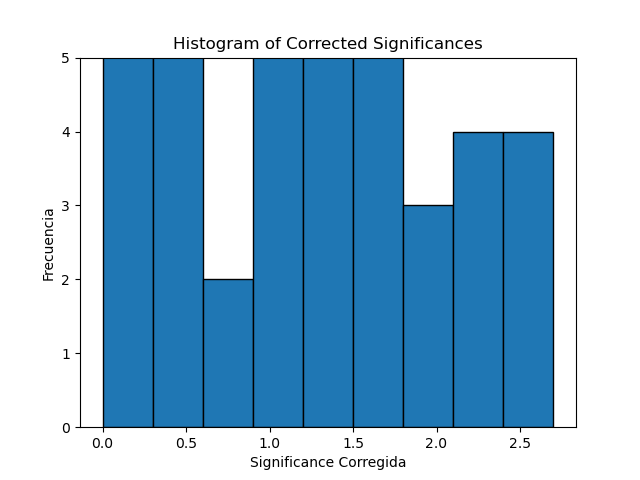
\includegraphics[width=0.6\textwidth]{corrected_significance_hist.png}
\caption{Histogram of Corrected Significances.}
\end{figure}

\section*{Conclusion}
The Fisher combined test integrates individual p-values to evaluate a global hypothesis.
The resulting test statistic was $X^2 = 317.927$ with 158 degrees of freedom.
For a significance level of 0.05, the critical value is 188.332.
Since $X^2$ is greater than the critical value, we rechazamos the null hypothesis of independence.
Normal approximation: p-value = 9.868e-13, significance ≈ 7.04 sigma.

\end{document}